\subsection{图的定义}

\begin{frame}\ft{\subsecname}
\begin{dingyi}
图是由顶点的有穷非空集合与定点之间边的集合组成的,通常表示为
$G(V,E)$,其中$G$表示一个图,$V$是图$G$中顶点的集合,$E$是图$G$中边的集合。
\end{dingyi}
\end{frame}


\begin{frame}\ft{\subsecname}

\begin{figure}
\centering
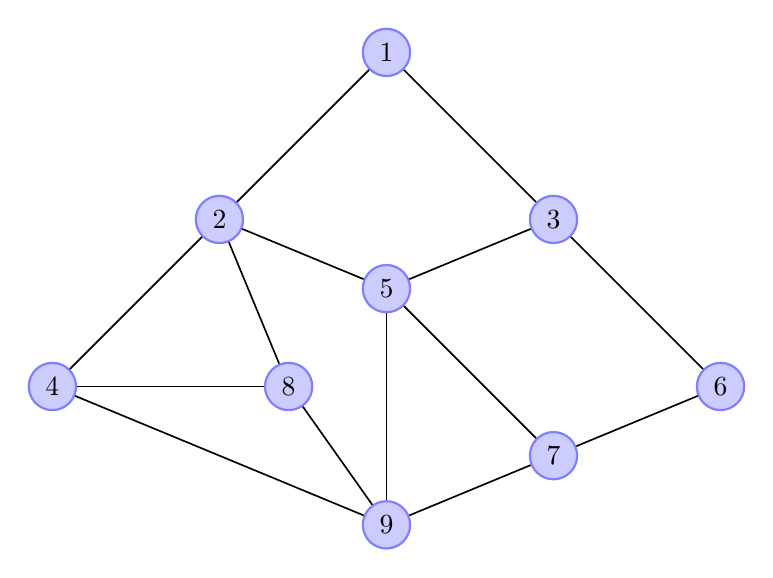
\begin{tikzpicture}[node distance=3cm,semithick,inner sep=1pt,bend angle=45,auto]
%\draw[help lines] (-3,-3) grid (3,0);
\node[state]   (v1)                     {1};
\node[state]   (v2) [below left  of=v1] {2};
\node[state]   (v3) [below right of=v1] {3};
\node[state]   (v4) [below left  of=v2] {4};
\node[state]   (v5) [below       of=v1] {5};
\node[state]   (v6) [below right of=v3] {6};
\node[state]   (v7) [below right of=v5] {7};
\node[state]   (v8) [right       of=v4] {8};
\node[state]   (v9) [below       of=v5] {9};

\path
(v1) edge node{} (v2)
     edge node{} (v3)
(v2) edge node{} (v4)
     edge node{} (v5)
     edge node{} (v8)
(v3) edge node{} (v5)
     edge node{} (v6)
(v4) edge node{} (v8)
     edge node{} (v9)
(v5) edge node{} (v7)
     edge node{} (v9)
(v6) edge node{} (v7)
(v7) edge node{} (v9)
(v8) edge node{} (v9);                     
\end{tikzpicture}
\end{figure}
\end{frame}




\begin{frame}\ft{\subsecname}
注意:
\begin{itemize}
\item 
\tf线性表中数据元素叫元素,树中数据元素叫结点,图中数据元素称之为顶点(vertex)。\\[0.1in]
\item 
线性表若无数据元素,称为空表。树中没有结点称为空树。但在图中,不允许没有顶点,即顶点集合$V$有穷非空。
\end{itemize}•
\end{frame}


\subsection{各种图的定义}
\begin{frame}\ft{\subsubsecname}
\begin{dingyi}[无向图]
\begin{itemize}
\item 
\tf若顶点$v_i$到$v_j$之间的边没有方向,则称这条边为无向边(edge),用无序偶对$(v_i,v_j)$表示。\\[0.1in]
\item
\tf若图中任意两顶点之间的边都是无向边,则称该图为无向图(undirected graphs)。
\end{itemize}
\end{dingyi}
\end{frame}

\begin{frame}\ft{\subsubsecname}
\begin{figure}
\centering
\tikzstyle{state}=[circle,draw=blue!50,fill=blue!20,thick,inner sep=0pt,minimum size=6mm]


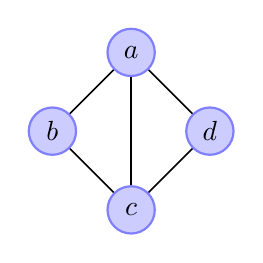
\begin{tikzpicture}[node distance=2cm,semithick,bend angle=45,minimum size=0.1cm,draw,auto]
\node[state]   (a) at  (90:1) {$a$};
\node[state]   (b) at (180:1) {$b$};
\node[state]   (c) at (270:1) {$c$};
\node[state]   (d) at   (0:1) {$d$};
\path
(a) edge (b)
    edge (c)   
    edge (d)
(b) edge (c)
(c) edge (d);             
\end{tikzpicture}
\caption{无向图}
\end{figure}
\end{frame}

\begin{frame}\ft{\subsubsecname}
\begin{dingyi}[有向图]
\begin{itemize}
\item 
\tf若顶点$v_i$到$v_j$之间的边有方向,则称这条边为有向边,也称为弧(arc),用有序偶对$<v_i,v_j>$表示,其中$v_i$称为弧尾(tail),$v_j$称为弧头(head)。\\[0.1in]
\item
\tf若图中任意两顶点之间的边都是有向边,则称该图为有向图(directed graphs)。
\end{itemize}
\end{dingyi}
\end{frame}


\begin{frame}\ft{\subsubsecname}
\begin{figure}
\centering
\tikzstyle{state}=[circle,draw=blue!50,fill=blue!20,thick,inner sep=0pt,minimum size=6mm]

\begin{tikzpicture}[->,>=stealth',shorten >=1pt,node distance=2cm,semithick,inner sep=1pt,bend angle=45,auto]
\node[state]   (A)                    {A};
\node[state]   (B) [below left  of=A] {B};
\node[state]   (C) [below right of=B] {C};
\node[state]   (D) [below right of=A] {D};
\path
(A) edge node{} (D)
(B) edge node{} (A)
    edge node{} (C)
(C) edge node{} (A);                     
\end{tikzpicture}
\caption{有向图}
\end{figure}
\end{frame}

\begin{frame}\ft{\subsubsecname}
\begin{dingyi}[简单图]
若不存在顶点到自身的边,且同一条边不重复出现,则称这样的图为简单图。
\end{dingyi}

\red{本章只讨论简单图。}

\begin{figure}
\centering
\tikzstyle{state}=[circle,draw=blue!50,fill=blue!20,thick,inner sep=0pt,minimum size=6mm]
\begin{minipage}{0.45\textwidth}
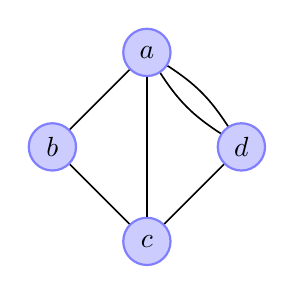
\begin{tikzpicture}[scale=1.2,node distance=3cm,semithick,inner sep=1pt,bend angle=45,auto]
%\draw[help lines] (-3,-3) grid (3,0);
\node[state]   (a) at  (90:1) {$a$};
\node[state]   (b) at (180:1) {$b$};
\node[state]   (c) at (270:1) {$c$};
\node[state]   (d) at   (0:1) {$d$};
\path
(a) edge (b)
    edge (c)   
    edge[bend left=12] (d)
	 edge[bend right=12](d)
(b) edge (c)
(c) edge (d);             
\end{tikzpicture}
\end{minipage}
%%%%%%%%
\begin{minipage}{0.45\textwidth}
\begin{tikzpicture}[scale=1.2,->,>=stealth',node distance=3cm,semithick,inner sep=1pt,bend angle=45,auto]
%\draw[help lines] (-3,-3) grid (3,0);
\node[state]   (a) at  (90:1) {$a$};
\node[state]   (b) at (180:1) {$b$};
\node[state]   (c) at (270:1) {$c$};
\node[state]   (d) at   (0:1) {$d$};
\path
(a) edge (d)   
    edge[loop above] (A)
(b) edge (a)
    edge (c)
(c) edge (a);             
\end{tikzpicture}
\end{minipage}

\caption{非简单无向图}
\end{figure}
\end{frame}


\begin{frame}\ft{\subsubsecname}
\begin{dingyi}[无向完全图]
在无向图中,若任意两顶点之间都存在边,则称该图为无向完全图。
\end{dingyi} \vspace{0.1in}

\red{含有$n$个顶点的无向完全图有$\frac{n(n-1)}2$条边。}

\begin{figure}
\centering
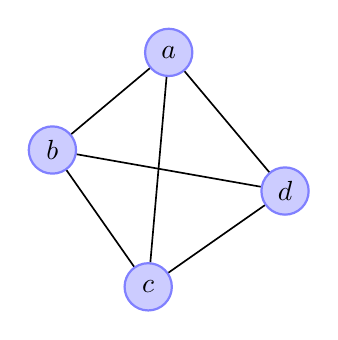
\begin{tikzpicture}[scale=1.5,node distance=3cm,semithick,bend angle=45,minimum size=0.1cm,draw,auto]
%\draw[help lines] (-3,-3) grid (3,0);
\node[state]   (a) at  (90:1) {$a$};
\node[state]   (b) at (170:1) {$b$};
\node[state]   (c) at (260:1) {$c$};
\node[state]   (d) at (350:1) {$d$};
\path
(a) edge (b)
    edge (c)   
    edge (d)
(b) edge (c)
    edge (d)
(c) edge (d);             
\end{tikzpicture}
\caption{无向完全图}
\end{figure}

\end{frame}


\begin{frame}\ft{\subsubsecname}
\begin{dingyi}[有向完全图]
在有向图中,若任意两顶点之间都存在方向相反的两条弧,则称该图为有向完全图。
\end{dingyi}\vspace{0.1in}

\red{含有$n$个顶点的有向完全图有$n(n-1)$条弧。}

\begin{figure}
\centering
\begin{tikzpicture}[scale=1.5,node distance=3cm,semithick,bend angle=45,minimum size=0.1cm,draw,auto]
%\draw[help lines] (-3,-3) grid (3,0);
\node[state]   (a) at  (90:1) {$a$};
\node[state]   (b) at (170:1) {$b$};
\node[state]   (c) at (260:1) {$c$};
\node[state]   (d) at (350:1) {$d$};
\path
(a) edge[->,>=stealth',bend left=10]  (b)
    edge[<-,>=stealth',bend right=10] (b)
    edge[->,>=stealth',bend left=10]  (c)
    edge[<-,>=stealth',bend right=10] (c) 
    edge[->,>=stealth',bend left=10]  (d)
    edge[<-,>=stealth',bend right=10] (d)
(b) edge[->,>=stealth',bend left=10]  (c)
    edge[<-,>=stealth',bend right=10] (c)
    edge[->,>=stealth',bend left=10]  (d)
    edge[<-,>=stealth',bend right=10] (d)
(c) edge[->,>=stealth',bend left=10]  (d)
    edge[<-,>=stealth',bend right=10] (d);             
\end{tikzpicture}
\caption{有向完全图}
\end{figure}

\end{frame}

\begin{frame}\ft{\subsubsecname}
对于具有$n$个顶点和$e$条边的图,无向图满足
$$
0\le e \le \frac{n(n-1)}2,
$$
有向图满足
$$
0\le e \le n(n-1).
$$
\end{frame}

\begin{frame}\ft{\subsubsecname}
\begin{dingyi}[稠密图与稀疏图]
有很少条边或弧的图称为稀疏图,反之称为稠密图。
\end{dingyi}\vspace{0.1in}

\red{这里稀疏与稠密是模糊概念,都是相对而言的。}
\end{frame}


\begin{frame}\ft{\subsubsecname}
\begin{dingyi}[网]
\begin{itemize}
\item
\tf有些图的边或弧具有与它相关的数字,这种与边或弧相关的数称为权(weight)。这些权可以表示从一个顶点到另一个顶点的距离或耗费。
\item
\tf这种带权的图称为网(network)。
\end{itemize}
\end{dingyi}

\begin{figure}
\centering
\tikzstyle{state}=[circle,draw=blue!50,fill=blue!20,thick,inner sep=0pt,minimum size=6mm]

\begin{tikzpicture}[scale=1.3,node distance=3cm,semithick,bend angle=45,minimum size=0.1cm,draw,auto]
%\draw[help lines] (-3,-3) grid (3,0);
\node[state]   (a) at (110:1.5) {北京};
\node[state]   (b) at (220:1.5) {香港};
\node[state]   (c) at (-45:1)   {台北};
\node[state]   (d) at  (45:1)   {上海};
\path
(a) edge node[near start,above]{\tiny 1463} (b)
    edge node[near start,below]{\tiny 2160}(c)   
    edge node[near start]{\tiny 1680}(d)
(b) edge node[near end,below]{\tiny  808}(c)
    edge node[midway,below]{\tiny 1200}(d)
(c) edge node[midway,right]{\tiny  700}(d);             
\end{tikzpicture}
\caption{网}
\end{figure}

\end{frame}


\begin{frame}\ft{\subsubsecname}
\begin{dingyi}[子图]
\tf假设有两个图$G=(V,E)$和$G^\prime=(V^\prime,E^\prime)$,如果$V^\prime\subset V$且$E^\prime\subset E$,则称$G^\prime$为$G$的子图(subgraph)。
\end{dingyi}
\end{frame}


\begin{frame}\ft{\subsubsecname}
\begin{figure}
\centering
\tikzstyle{state}=[circle,draw=blue!50,fill=blue!20,thick,inner sep=0pt,minimum size=6mm]

\begin{minipage}{\textwidth}
\begin{minipage}{0.35\textwidth}
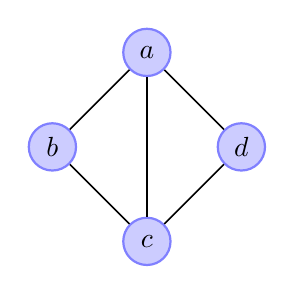
\begin{tikzpicture}[scale=1.2,node distance=3cm,semithick,inner sep=1pt,bend angle=45,auto]
%\draw[help lines] (-3,-3) grid (3,0);
\node[state]   (a) at  (90:1) {$a$};
\node[state]   (b) at (180:1) {$b$};
\node[state]   (c) at (270:1) {$c$};
\node[state]   (d) at   (0:1) {$d$};
\path
(a) edge (b)
    edge (c)   
    edge (d)
(b) edge (c)
(c) edge (d);             
\end{tikzpicture}
\end{minipage}
%%%%%
\begin{minipage}{0.1\textwidth}
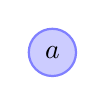
\begin{tikzpicture}[scale=1.2,node distance=3cm,semithick,inner sep=1pt,bend angle=45,auto]
%\draw[help lines] (-3,-3) grid (3,0);
\node[state]   (a) at  (90:1) {$a$};            
\end{tikzpicture}
\end{minipage}
%%%%%
\begin{minipage}{0.25\textwidth}
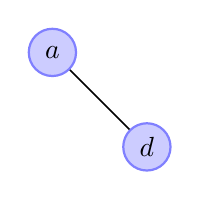
\begin{tikzpicture}[scale=1.2,node distance=3cm,semithick,inner sep=1pt,bend angle=45,auto]
%\draw[help lines] (-3,-3) grid (3,0);
\node[state]   (a) at  (90:1) {$a$};
\node[state]   (d) at   (0:1) {$d$};
\path
(a) edge (d);             
\end{tikzpicture}
\end{minipage}
%%%%%
\begin{minipage}{0.25\textwidth}
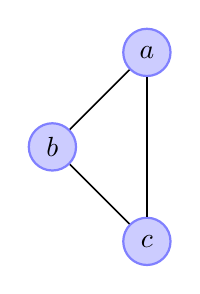
\begin{tikzpicture}[scale=1.2,node distance=3cm,semithick,inner sep=1pt,bend angle=45,auto]
%\draw[help lines] (-3,-3) grid (3,0);
\node[state]   (a) at  (90:1) {$a$};
\node[state]   (b) at (180:1) {$b$};
\node[state]   (c) at (270:1) {$c$};
\path
(a) edge (b)
    edge (c)   
(b) edge (c);
\end{tikzpicture}
\end{minipage}
\end{minipage} \vspace{0.05in}

%%%%%%%%
%%%%%%%%
\begin{minipage}{\textwidth}
\begin{minipage}{0.35\textwidth}
\begin{tikzpicture}[scale=1.2,->,>=stealth',node distance=3cm,semithick,inner sep=1pt,bend angle=45,auto]
%\draw[help lines] (-3,-3) grid (3,0);
\node[state]   (a) at  (90:1) {$a$};
\node[state]   (b) at (180:1) {$b$};
\node[state]   (c) at (270:1) {$c$};
\node[state]   (d) at   (0:1) {$d$};
\path
(a) edge (d)   
(b) edge (a)
    edge (c)
(c) edge (a);             
\end{tikzpicture}
\end{minipage}
%%%%
\begin{minipage}{0.1\textwidth}
\begin{tikzpicture}[scale=1.2,->,>=stealth',node distance=3cm,semithick,inner sep=1pt,bend angle=45,auto]
%\draw[help lines] (-3,-3) grid (3,0);
\node[state]   (a) at  (90:1) {$a$};           
\end{tikzpicture}
\end{minipage}
%%%%
\begin{minipage}{0.25\textwidth}
\begin{tikzpicture}[scale=1.2,->,>=stealth',node distance=3cm,semithick,inner sep=1pt,bend angle=45,auto]
%\draw[help lines] (-3,-3) grid (3,0);
\node[state]   (a) at  (90:1) {$a$};
\node[state]   (d) at   (0:1) {$d$};
\path
(a) edge (d);             
\end{tikzpicture}
\end{minipage}
\begin{minipage}{0.25\textwidth}
\begin{tikzpicture}[scale=1.2,->,>=stealth',node distance=3cm,semithick,inner sep=1pt,bend angle=45,auto]
%\draw[help lines] (-3,-3) grid (3,0);
\node[state]   (a) at  (90:1) {$a$};
\node[state]   (b) at (180:1) {$b$};
\node[state]   (c) at (270:1) {$c$};
\path
(b) edge (a)
    edge (c)
(c) edge (a);             
\end{tikzpicture}
\end{minipage}
\end{minipage}

\caption{子图}
\end{figure}

\end{frame}

\subsection{顶点与边之间的关系}

\begin{frame}\ft{\subsubsecname}
\begin{dingyi}[无向图顶点的邻接、度]
对于无向图$G=(V,E)$,
\begin{itemize}
\item 
\tf若边$(v,v^\prime)\in E$,则称顶点$v$与$v^\prime$互为邻接点(adjacent),边$(v,v^\prime)$与顶点$v$和$v^\prime$相关联。 \\[0.1in]
\item 
\tf顶点$v$的度(degree)是和$v$相关联的边的数目,记为$\TD(v)$。\\[0.1in]
\item 重要关系:
$$
e=\frac12 \sum_{i=1}^n \TD(v_i).
$$
\end{itemize}
\end{dingyi}
\end{frame}

\begin{frame}\ft{\subsubsecname}
\begin{dingyi}[有向图顶点的邻接、入度、出度和度]
对于有向图$G=(V,E)$,
\begin{itemize}
\item 
\tf若弧$<v,v^\prime>\in E$,则称顶点$v$邻接到顶点$v^\prime$,顶点$v^\prime$邻接于$v$,弧$<v,v^\prime>$与顶点$v,v^\prime$相关联。 \\[0.1in]
\item 
\tf以顶点$v$为头的弧的数目称为$v$的入度(indegree),记为$\ID(v)$;

以顶点$v$为尾的弧的数目称为$v$的出度(outdegree),记为$\OD(v)$;

顶点$v$的度为$\TD(v)=\ID(v)+\OD(v)$。\\[0.1in]
\item 重要关系:
$$
e=\sum_{i=1}^n \ID(v_i)=\sum_{i=1}^n \OD(v_i).
$$
\end{itemize}
\end{dingyi}
\end{frame}

\begin{frame}\ft{\subsubsecname}
\begin{dingyi}[无向图的路径]
\tf对于无向图$G=(V,E)$,从顶点$v$到顶点$v^\prime$的路径(path)是一个顶点序列$(v=v_{i_0}, v_{i_1}, \cd, v_{i_m}=v^\prime)$,其中$(v_{i_{k-1}},v_{i_{k}})\in E, ~1\le k \le m$。
\end{dingyi}
\end{frame}

\begin{frame}\ft{\subsubsecname}
\begin{figure}
\centering
\begin{minipage}{0.45\textwidth}
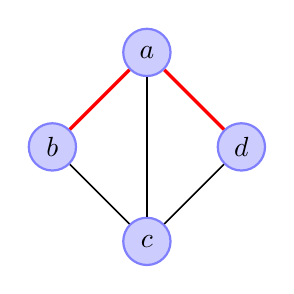
\begin{tikzpicture}[scale=1.2,node distance=3cm,semithick,inner sep=1pt,bend angle=45,auto]
%\draw[help lines] (-3,-3) grid (3,0);
\node[state]   (a) at  (90:1) {$a$};
\node[state]   (b) at (180:1) {$b$};
\node[state]   (c) at (270:1) {$c$};
\node[state]   (d) at   (0:1) {$d$};
\path
(a) edge[very thick,red] (b)
    edge (c)   
    edge[very thick,red] (d)
(b) edge (c)
(c) edge (d);             
\end{tikzpicture}
\end{minipage}
%%%%%
\begin{minipage}{0.45\textwidth}
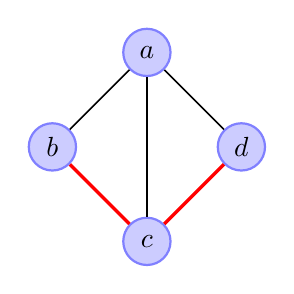
\begin{tikzpicture}[scale=1.2,node distance=3cm,semithick,inner sep=1pt,bend angle=45,auto]
%\draw[help lines] (-3,-3) grid (3,0);
\node[state]   (a) at  (90:1) {$a$};
\node[state]   (b) at (180:1) {$b$};
\node[state]   (c) at (270:1) {$c$};
\node[state]   (d) at   (0:1) {$d$};
\path
(a) edge (b)
    edge (c)   
    edge (d)
(b) edge[very thick,red] (c)
(c) edge[very thick,red] (d);             
\end{tikzpicture}
\end{minipage} \vspace{0.1in}



\begin{minipage}{0.45\textwidth}
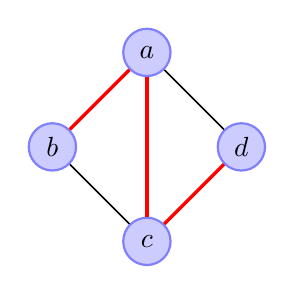
\begin{tikzpicture}[scale=1.2,node distance=3cm,semithick,inner sep=1pt,bend angle=45,auto]
%\draw[help lines] (-3,-3) grid (3,0);
\node[state]   (a) at  (90:1) {$a$};
\node[state]   (b) at (180:1) {$b$};
\node[state]   (c) at (270:1) {$c$};
\node[state]   (d) at   (0:1) {$d$};
\path
(a) edge[very thick,red] (b)
    edge[very thick,red] (c)   
    edge (d)
(b) edge (c)
(c) edge[very thick,red] (d);             
\end{tikzpicture}
\end{minipage}
%%%%%
\begin{minipage}{0.45\textwidth}
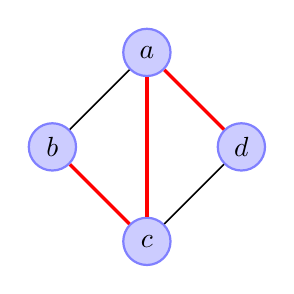
\begin{tikzpicture}[scale=1.2,node distance=3cm,semithick,inner sep=1pt,bend angle=45,auto]
%\draw[help lines] (-3,-3) grid (3,0);
\node[state]   (a) at  (90:1) {$a$};
\node[state]   (b) at (180:1) {$b$};
\node[state]   (c) at (270:1) {$c$};
\node[state]   (d) at   (0:1) {$d$};
\path
(a) edge (b)
    edge[very thick,red] (c)   
    edge[very thick,red] (d)
(b) edge[very thick,red] (c)
(c) edge (d);             
\end{tikzpicture}
\end{minipage}

\caption{顶点$b$到$d$有四条路径}
\end{figure}

\end{frame}

\begin{frame}\ft{\subsubsecname} 
\begin{dingyi}[有向图的路径]
\tf对于有向图$G=(V,E)$,其路径也是有向的,顶点序列应满足$(v_{i_{k-1}},v_{i_{k}})\in E, ~1\le k \le m$。
\end{dingyi}
\end{frame}


\begin{frame}\ft{\subsubsecname}
\begin{figure}
\centering
\begin{minipage}{0.45\textwidth}
\begin{tikzpicture}[scale=1.2,->,>=stealth',node distance=3cm,semithick,inner sep=1pt,bend angle=45,auto]
%\draw[help lines] (-3,-3) grid (3,0);
\node[state]   (a) at  (90:1) {$a$};
\node[state]   (b) at (180:1) {$b$};
\node[state]   (c) at (270:1) {$c$};
\node[state]   (d) at   (0:1) {$d$};
\path
(a) edge[very thick,red]  (d)   
(b) edge[very thick,red]  (a)
    edge (c)
(c) edge (a);             
\end{tikzpicture}
\end{minipage}
%%%%%
\begin{minipage}{0.45\textwidth}
\begin{tikzpicture}[scale=1.2,->,>=stealth',node distance=3cm,semithick,inner sep=1pt,bend angle=45,auto]
%\draw[help lines] (-3,-3) grid (3,0);
\node[state]   (a) at  (90:1) {$a$};
\node[state]   (b) at (180:1) {$b$};
\node[state]   (c) at (270:1) {$c$};
\node[state]   (d) at   (0:1) {$d$};
\path
(a) edge[very thick,red]  (d)   
(b) edge (a)
    edge[very thick,red]  (c)
(c) edge[very thick,red]  (a);             
\end{tikzpicture}
\end{minipage}



\caption{顶点$b$到$d$有两条路径}
\end{figure}
\end{frame}


\begin{frame}\ft{\subsubsecname} 
\begin{dingyi}[路径长度]
\tf路径的长度是路径上的边或弧的数目。
\end{dingyi}
\end{frame}

\begin{frame}\ft{\subsubsecname}
\begin{dingyi}[回路或环]
\tf第一个顶点和最后一个顶点相同的路径称为回路或环(cycle)。
\end{dingyi}
%\pause 
\begin{dingyi}[简单路径]
\tf序列中顶点不重复出现的路径称为简单路径。
\end{dingyi}
%\pause 
\begin{dingyi}[简单回路或简单环]
\tf除第一个顶点和最后一个顶点外,其余顶点不重复的回路,称为简单回路或简单环。
\end{dingyi}

\end{frame}

\begin{frame}\ft{\subsubsecname}
\begin{figure}
\centering
\begin{minipage}{0.45\textwidth}
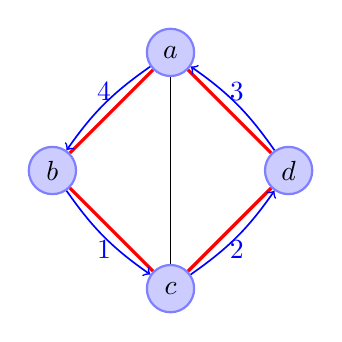
\begin{tikzpicture}[scale=1.5,node distance=3cm,semithick,inner sep=1pt,bend angle=45,auto]
%\draw[help lines] (-3,-3) grid (3,0);
\node[state]   (a) at  (90:1) {$a$};
\node[state]   (b) at (180:1) {$b$};
\node[state]   (c) at (270:1) {$c$};
\node[state]   (d) at   (0:1) {$d$};
\path
(a) edge[very thick,red](b) edge[->,above,blue,bend right=10]node{4}(b)
    edge(c)   
    edge[very thick,red](d) edge[<-,above,blue,bend left=10]node{3}(d)
(b) edge[very thick,red](c) edge[->,below,blue,bend right=10]node{1} (c)
(c) edge[very thick,red](d) edge[->,below,blue,bend right=10]node{2} (d);             
\end{tikzpicture}
\caption{简单回路}
\end{minipage}
%%%%%
\begin{minipage}{0.45\textwidth}
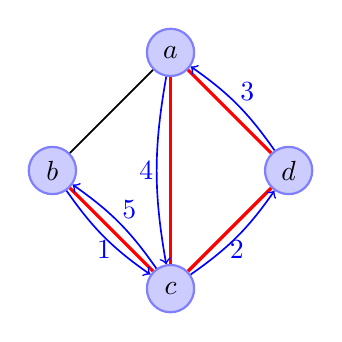
\begin{tikzpicture}[scale=1.5,node distance=3cm,semithick,inner sep=1pt,bend angle=45,auto]
%\draw[help lines] (-3,-3) grid (3,0);
\node[state]   (a) at  (90:1) {$a$};
\node[state]   (b) at (180:1) {$b$};
\node[state]   (c) at (270:1) {$c$};
\node[state]   (d) at   (0:1) {$d$};
\path
(a)edge (b)
   edge[very thick,red](c) edge[->,blue,bend right=10]node[left]{4}(c)   
   edge[very thick,red](d) edge[<-,blue,bend left=10]node{3}(d)
(b)edge[very thick,red](c) edge[->,blue,bend right=10]node[below]{1}(c) edge[<-,blue,bend left=10]node{5}(c)
(c)edge[very thick,red](d) edge[->,blue,bend right=10]node[below]{2}(d);             
\end{tikzpicture}
\caption{非简单回路}
\end{minipage}  


\end{figure}
\end{frame}


\subsection{连通图}

\begin{frame}\ft{\subsubsecname}
\begin{dingyi}[连通图]
\begin{itemize}
\item 
在无向图中,若顶点$v$到$v^\prime$有路径,则称$v$与$v^\prime$是连通的。 \\[0.1in]
\item
\tf若对任意两个顶点$v_i,v_j\in E$,$v_i$和$v_j$都是连通的,则称$G$是连通图(connected graph)。
\end{itemize}
\end{dingyi}
\begin{figure}
\centering
\begin{minipage}{0.45\textwidth}
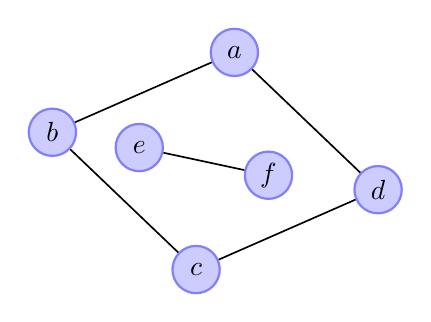
\begin{tikzpicture}[scale=1.4,node distance=3cm,semithick,inner sep=1pt,bend angle=45,auto]
%\draw[help lines] (-3,-3) grid (3,0);
\node[state]   (a) at  (80:1) {$a$};
\node[state]   (b) at (170:1.5) {$b$};
\node[state]   (c) at (260:1) {$c$};
\node[state]   (d) at  (-10:1.5) {$d$};
\node[state]   (e) at (170:0.7) {$e$};
\node[state]   (f) at  (-15:0.5) {$f$};
\path
(a) edge (b)  
    edge (d)  
(b) edge (c) 
(c) edge (d)
(e) edge (f) ;             
\end{tikzpicture}
\caption{非连通图}
\end{minipage}
%%%%%
\begin{minipage}{0.45\textwidth}
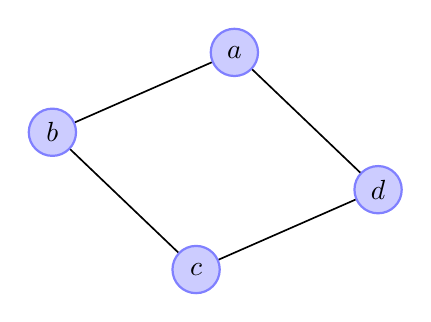
\begin{tikzpicture}[scale=1.4,node distance=3cm,semithick,inner sep=1pt,bend angle=45,auto]
%\draw[help lines] (-3,-3) grid (3,0);
\node[state]   (a) at  (80:1) {$a$};
\node[state]   (b) at (170:1.5) {$b$};
\node[state]   (c) at (260:1) {$c$};
\node[state]   (d) at  (-10:1.5) {$d$};
\path
(a) edge (b)  
    edge (d)  
(b) edge (c) 
(c) edge (d) ;             
\end{tikzpicture}
\caption{连通图}
\end{minipage}  


\end{figure}

\end{frame}


\begin{frame}\ft{\subsubsecname}
\begin{dingyi}[连通分量]
无向图中的极大连通子图称为连通分量。
\end{dingyi} %\pause 
\vspace{0.1in}

此概念强调\\[0.03in]
\begin{itemize}
\item 
要是子图; \\[0.1in]
\item
子图要是连通的;\\[0.1in]
\item
连通子图含有极大顶点数;\\[0.1in]
\item
具有极大顶点数的连通子图包含相关联于这些顶点的边。
\end{itemize}
\end{frame}


\begin{frame}\ft{\subsubsecname}
\begin{figure}
\centering
\begin{minipage}{0.45\textwidth}
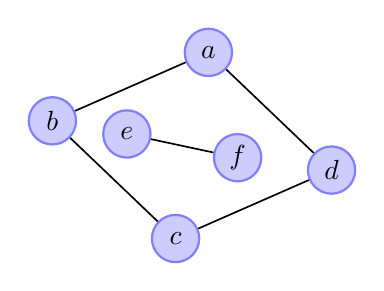
\begin{tikzpicture}[scale=1.2,node distance=3cm,semithick,inner sep=1pt,bend angle=45,auto]
%\draw[help lines] (-3,-3) grid (3,0);
\node[state]   (a) at  (80:1) {$a$};
\node[state]   (b) at (170:1.5) {$b$};
\node[state]   (c) at (260:1) {$c$};
\node[state]   (d) at  (-10:1.5) {$d$};
\node[state]   (e) at (170:0.7) {$e$};
\node[state]   (f) at  (-15:0.5) {$f$};
\path
(a) edge (b)  
    edge (d)  
(b) edge (c) 
(c) edge (d)
(e) edge (f) ;             
\end{tikzpicture}
\caption{非连通图}
\end{minipage}
%%%%%
\begin{minipage}{0.45\textwidth}
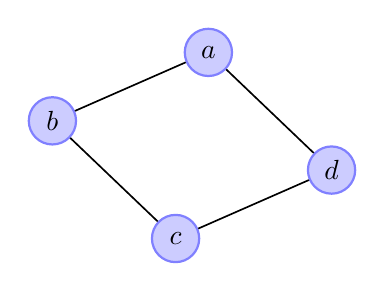
\begin{tikzpicture}[scale=1.2,node distance=3cm,semithick,inner sep=1pt,bend angle=45,auto]
%\draw[help lines] (-3,-3) grid (3,0);
\node[state]   (a) at  (80:1) {$a$};
\node[state]   (b) at (170:1.5) {$b$};
\node[state]   (c) at (260:1) {$c$};
\node[state]   (d) at  (-10:1.5) {$d$};
\path
(a) edge (b)  
    edge (d)  
(b) edge (c) 
(c) edge (d) ;             
\end{tikzpicture}
\caption{连通分量}
\end{minipage}  

\begin{minipage}{0.45\textwidth}
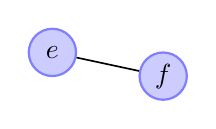
\begin{tikzpicture}[scale=1.2,node distance=3cm,semithick,inner sep=1pt,bend angle=45,auto]
%\draw[help lines] (-3,-3) grid (3,0);
\node[state]   (e) at (170:0.7) {$e$};
\node[state]   (f) at  (-15:0.5) {$f$};
\path
(e) edge (f) ;         
\end{tikzpicture}
\caption{连通分量}
\end{minipage}
%%%%%
\begin{minipage}{0.45\textwidth}
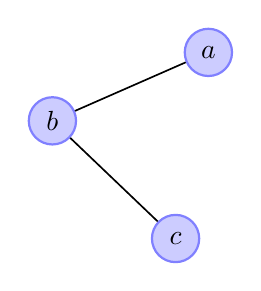
\begin{tikzpicture}[scale=1.2,node distance=3cm,semithick,inner sep=1pt,bend angle=45,auto]
%\draw[help lines] (-3,-3) grid (3,0);
\node[state]   (a) at  (80:1) {$a$};
\node[state]   (b) at (170:1.5) {$b$};
\node[state]   (c) at (260:1) {$c$};
\path
(a) edge (b)  
(b) edge (c);             
\end{tikzpicture}
\caption{不是连通分量}
\end{minipage} 


\end{figure}
\end{frame}


\begin{frame}\ft{\subsubsecname}
\begin{dingyi}
在有向图$G$中,若对每一对$v_i,v_j\in V, v_i\ne v_j$,从$v_i$到$v_j$和从$v_j$到$v_i$存在路径,则称$G$是强连通图。有向图中的极大强连通子图称为有向图的强连通分量。
\end{dingyi}
\end{frame}

\begin{frame}\ft{\subsubsecname}
\begin{figure}
\centering
\begin{minipage}{0.45\textwidth}
\begin{tikzpicture}[scale=1.2,->,>=stealth',node distance=3cm,semithick,inner sep=1pt,bend angle=45,auto]
%\draw[help lines] (-3,-3) grid (3,0);
\node[state]   (a) at  (90:1) {$a$};
\node[state]   (b) at (180:1) {$b$};
\node[state]   (c) at (270:1) {$c$};
\node[state]   (d) at   (0:1) {$d$};
\path
(a) edge (d) 
    edge (b)   
(b) edge (c)
(c) edge (a);             
\end{tikzpicture}
\caption{非强连通图}
\end{minipage}
%%%%%
\begin{minipage}{0.45\textwidth}
\begin{tikzpicture}[scale=1.2,->,>=stealth',node distance=3cm,semithick,inner sep=1pt,bend angle=45,auto]
%\draw[help lines] (-3,-3) grid (3,0);
\node[state]   (a) at  (90:1) {$a$};
\node[state]   (b) at (180:1) {$b$};
\node[state]   (c) at (270:1) {$c$};
\path
(a) edge (b)   
(b) edge (c)
(c) edge (a);            
\end{tikzpicture}
\caption{强连通分量}
\end{minipage}



\end{figure}
\end{frame}


\begin{frame}\ft{\subsubsecname}
\begin{dingyi}[连通图的生成树]
一个连通图的生成子树是一个极小的连通子图,它含有图中全部的$n$个顶点,但只有足以构成一棵树的$n-1$条边。
\end{dingyi}%\pause
\vspace{0.1in}

设无向图$G$有$n$个顶点,\\[0.05in]
\begin{itemize}
\item
若边数小于$n-1$,则$G$是非连通图;\\[0.1in]
\item
若边数大于$n-1$,则$G$必定构成一个环;\\[0.1in]
\item
但边数等于$n-1$,并不一定是生成树。
\end{itemize}
\end{frame}

\begin{frame}\ft{\subsubsecname}
\begin{figure}
\centering

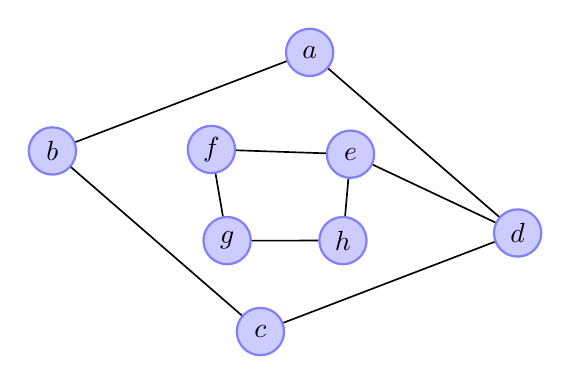
\begin{tikzpicture}[scale=1.2,node distance=3cm,semithick,inner sep=1pt,bend angle=45,auto]
%\draw[help lines] (-3,-3) grid (3,0);
\node[state]   (a) at  (80:1.5) {$a$};
\node[state]   (b) at (170:2.5) {$b$};
\node[state]   (c) at (260:1.5) {$c$};
\node[state]   (d) at  (-10:2.5) {$d$};
\node[state]   (e) at (30:0.8) {$e$};
\node[state]   (f) at  (150:0.9) {$f$};
\node[state]   (g) at (220:0.8) {$g$};
\node[state]   (h) at  (320:0.8) {$h$};
\path
(a) edge (b)  
    edge (d)  
(b) edge (c) 
(c) edge (d)
(e) edge (f) 
    edge (d)
    edge (h)
(f) edge (g)
(g) edge (h);             
\end{tikzpicture}


\caption{普通无向图}
\end{figure}
\end{frame}

\begin{frame}\ft{\subsubsecname}
\begin{figure}
\centering

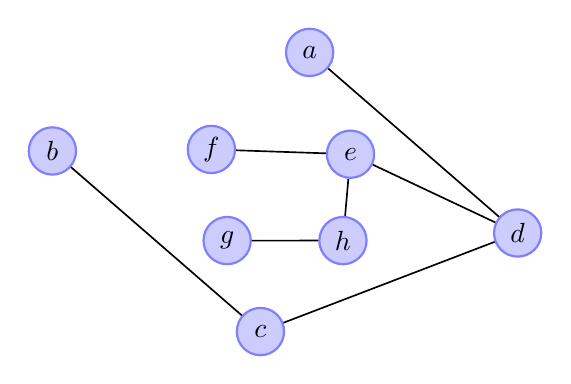
\begin{tikzpicture}[scale=1.2,node distance=3cm,semithick,inner sep=1pt,bend angle=45,auto]
%\draw[help lines] (-3,-3) grid (3,0);
\node[state]   (a) at  (80:1.5) {$a$};
\node[state]   (b) at (170:2.5) {$b$};
\node[state]   (c) at (260:1.5) {$c$};
\node[state]   (d) at  (-10:2.5) {$d$};
\node[state]   (e) at (30:0.8) {$e$};
\node[state]   (f) at  (150:0.9) {$f$};
\node[state]   (g) at (220:0.8) {$g$};
\node[state]   (h) at  (320:0.8) {$h$};
\path
(a) edge (d)  
(b) edge (c) 
(c) edge (d)
(e) edge (f) 
    edge (d)
    edge (h)
(g) edge (h);             
\end{tikzpicture}


\caption{无向图的生成树}
\end{figure}
\end{frame}


\begin{frame}\ft{\subsubsecname}
\begin{figure}
\centering

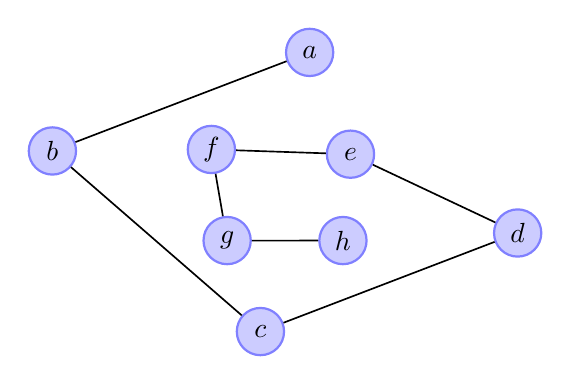
\begin{tikzpicture}[scale=1.2,node distance=3cm,semithick,inner sep=1pt,bend angle=45,auto]
%\draw[help lines] (-3,-3) grid (3,0);
\node[state]   (a) at  (80:1.5) {$a$};
\node[state]   (b) at (170:2.5) {$b$};
\node[state]   (c) at (260:1.5) {$c$};
\node[state]   (d) at  (-10:2.5) {$d$};
\node[state]   (e) at (30:0.8) {$e$};
\node[state]   (f) at  (150:0.9) {$f$};
\node[state]   (g) at (220:0.8) {$g$};
\node[state]   (h) at  (320:0.8) {$h$};
\path
(a) edge (b)  
(b) edge (c) 
(c) edge (d)
(e) edge (f) 
    edge (d)
(f) edge (g)
(g) edge (h);             
\end{tikzpicture}


\caption{无向图的生成树}
\end{figure}
\end{frame}

\begin{frame}\ft{\subsubsecname}
\begin{figure}
\centering

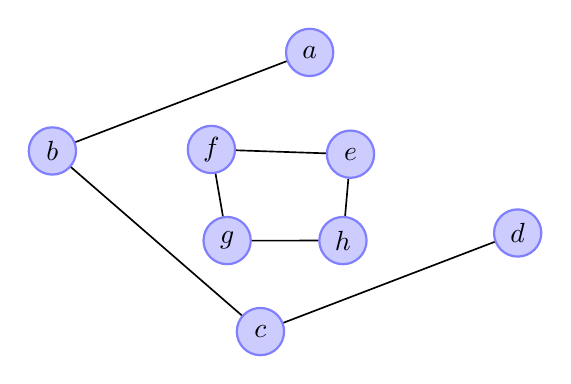
\begin{tikzpicture}[scale=1.2,node distance=3cm,semithick,inner sep=1pt,bend angle=45,auto]
%\draw[help lines] (-3,-3) grid (3,0);
\node[state]   (a) at  (80:1.5) {$a$};
\node[state]   (b) at (170:2.5) {$b$};
\node[state]   (c) at (260:1.5) {$c$};
\node[state]   (d) at  (-10:2.5) {$d$};
\node[state]   (e) at (30:0.8) {$e$};
\node[state]   (f) at  (150:0.9) {$f$};
\node[state]   (g) at (220:0.8) {$g$};
\node[state]   (h) at  (320:0.8) {$h$};
\path
(a) edge (b)  
(b) edge (c) 
(c) edge (d)
(e) edge (f) 
    edge (h)
(f) edge (g)
(g) edge (h);             
\end{tikzpicture}


\caption{不是生成树}
\end{figure}
\end{frame}


\begin{frame}\ft{\subsubsecname}
\begin{dingyi}[有向树的生成森林]
\begin{itemize}
\item\tf如果一个有向图恰有一个顶点的入度为0,其余顶点的入度均为1,则它是一棵有向树。\\[0.1in]
\item
一个有向图的生成森林由若干棵有向树组成,含有图中全部顶点,但只有足以构成若干棵不相交的有向树的弧。
\end{itemize}•
\end{dingyi}
\end{frame}


\begin{frame}\ft{\subsubsecname}
\begin{figure}
\centering

\begin{tikzpicture}[scale=1.2,->,>=stealth',node distance=3cm,semithick,inner sep=1pt,bend angle=45,auto]
%\draw[help lines] (-3,-3) grid (3,0);
\node[state]   (a) at (135:1.5) {$a$};
\node[state]   (b) at (180:2.3) {$b$};
\node[state]   (c) at (225:1.8) {$c$};
\node[state]   (d) at     (0:0) {$d$};
\node[state]   (e) at  (45:1.8) {$e$};
\node[state]   (f) at (350:2.5) {$f$};
\node[state]   (g) at (315:1.5) {$g$};
\path
(b) edge (a)  
    edge (c) 
(a) edge (d)
(c) edge (a)
(e) edge (d)
    edge (g) 
(f) edge (e)
    edge (g)
(g) edge (c)
    edge (d);
\end{tikzpicture}


\caption{普通有向树}
\end{figure}
\end{frame}

\begin{frame}\ft{\subsubsecname}
\begin{figure}
\centering

\begin{tikzpicture}[scale=1.2,->,>=stealth',node distance=3cm,semithick,inner sep=1pt,bend angle=45,auto]
%\draw[help lines] (-3,-3) grid (3,0);
\node[state]   (a) at (135:1.5) {$a$};
\node[state]   (b) at (180:2.3) {$b$};
\node[state]   (c) at (225:1.8) {$c$};
\node[state]   (d) at     (0:0) {$d$};
\node[state]   (e) at  (45:1.8) {$e$};
\node[state]   (f) at (350:2.5) {$f$};
\node[state]   (g) at (315:1.5) {$g$};
\path
(b) edge (a)  
    edge (c) 
(a) edge (d)

(f) edge (e)
    edge (g);
\end{tikzpicture}


\caption{有向树的生成森林}
\end{figure}
\end{frame}


\subsection{小结}
\begin{frame}\ft{\subsubsecname}
\begin{itemize}
\item 图按有无方向分为\red{无向图}和\red{有向图}。无向图由顶点和边构成,有向图由顶点和弧构成,弧有弧尾和弧头之分。\\[0.1in]
\item 图按照边或弧的多少分为\red{稀疏图}和\red{稠密图}。如果任意两顶点之间都存在边叫\red{完全图},有向的叫\red{有向完全图}。若无重复的边和顶点到自身的边则叫\red{简单图}。\\[0.1in]
\item 图中顶点之间有邻接、依附的概念。无向图顶点的边数叫做\blue{度},有向图顶点有\blue{入度}和\blue{出度}之分。\\[0.1in]
\item 带权的图称为\red{网}。

\end{itemize}•
\end{frame}

\begin{frame}\ft{\subsubsecname}
\begin{itemize}
\item 图中顶点间存在\blue{路径},两顶点存在路径则说明两顶点\blue{连通},如果路径最终回到起始点则称为\blue{环},当中不重复叫\blue{简单路径}。若任意两顶点都连通,则图就是\red{连通图},有向则称\red{强连通图}。图中有子图,若子图极大连通则为\blue{连通分量},有向的则称\blue{强连通分量}。\\[0.1in]
\item 无向图中连通且含有$n$个顶点$n-1$条边的子图叫\blue{生成树}。有向图中一顶点入度为0其余顶点入度为1的叫\blue{有向树},一个有向图由若干棵有向树构成\blue{生成森林}。

\end{itemize}•
\end{frame}

